% !TeX root = chapter3_2d_ixaru.tex
% !TeX root = thesis.tex
\ifdefined\UtilIncluded
  \renewcommand{\startchapter}[1]{}
  \renewcommand{\stopchapter}{}
  \renewcommand{\undefinedlabel}[2]{}
\else

\newcommand{\startchapter}[1]{\begin{document}\setcounter{chapter}{#1}\addtocounter{chapter}{-1}}
\newcommand{\stopchapter}{\printbibliography[title=Bibliography,heading=bibintoc]\end{document}}


\documentclass{book}
\usepackage[utf8]{inputenc}


\usepackage{geometry}
\geometry{
  papersize={170mm,240mm},
}

\usepackage{amsfonts,amsmath, amsthm, amssymb, mathtools}
\usepackage{xspace}
\usepackage[hidelinks,bookmarks,pdfusetitle]{hyperref}
\usepackage{listings}
\usepackage[pdftex]{graphicx}
\usepackage{bm}
\usepackage[english]{babel}
\usepackage{caption}
\usepackage{subcaption}
\usepackage[usenames,dvipsnames]{xcolor}
\usepackage{physics}
\usepackage{multicol}
\usepackage{xstring}
\usepackage{pythonhighlight}
\usepackage{parskip}
\usepackage{thmtools}
\usepackage{relsize}
\usepackage{bookmark}
\usepackage{lmodern}
\usepackage{ifthen}
\usepackage{biblatex}
\usepackage{microtype}
\usepackage{csquotes}
\usepackage{numprint}
\usepackage{mleftright}
\npthousandsep{{\ifmmode\mskip2mu\else\hskip0.2em\fi}}
\npdecimalsign{.}

\addbibresource{references.bib}

\newtheorem{theorem}{Theorem}[chapter]
\newtheorem{lemma}[theorem]{Lemma}
\newtheorem{corollary}[theorem]{Corollary}
\newtheorem{definition}[theorem]{Definition}

\DeclareRobustCommand{\oneD}{{1{\relsize{-1}D}}\xspace}
\DeclareRobustCommand{\twoD}{{2{\relsize{-1}D}}\xspace}
\DeclareRobustCommand{\threeD}{{3{\relsize{-1}D}}\xspace}
\DeclareRobustCommand{\cpp}{{{C\nolinebreak[4]\hspace{-.05em}\raisebox{.4ex}{\relsize{-3}\textbf{++}}}\xspace}}
\pdfstringdefDisableCommands{%
  \def\cpp{C++}%
  \def\oneD{1D}%
  \def\twoD{2D}%
  \def\threeD{3D}%
}

\newcommand{\longchapter}[2][]{%
  \chapter[#2]{#2}%
  \ifthenelse{\equal{#1}{}}{}{\chaptermark{#1}}}

\newcommand{\NN}{\mathbb{N}}
\newcommand{\ZZ}{\mathbb{Z}}
\newcommand{\QQ}{\mathbb{Q}}
\newcommand{\QQbar}{\overline{\mathbb{Q}}}
\newcommand{\RR}{\mathbb{R}}
\newcommand{\CC}{\mathbb{C}}

\newcommand{\Eigen}{\texttt{Eigen}}

\newcommand{\sage}{\texttt{sage}\xspace}

\newcommand{\hamiltonian}{\mathcal{H}}

\newcommand{\transposesign}{\intercal}
\newcommand{\transpose}[1]{{#1}^\transposesign}
\newcommand{\adjointsign}{\text{H}}
\newcommand{\adjoint}[1]{{#1}^\adjointsign}

\newcommand{\xmin}{{x_{\text{min}}}}
\newcommand{\xmax}{{x_{\text{max}}}}
\newcommand{\ymin}{{y_{\text{min}}}}
\newcommand{\ymax}{{y_{\text{max}}}}

\newcommand{\Cbottom}{\vb{C}_\text{bottom}}
\newcommand{\Ctop}{\vb{C}_\text{top}}
\newcommand{\ubottom}{\vb{u}_\text{bottom}}
\newcommand{\utop}{\vb{u}_\text{top}}

\DeclareMathOperator{\diag}{diag}
\DeclareMathOperator{\tridiag}{tridiag}
\DeclareMathOperator{\eigs}{eigs}
\DeclareMathOperator*{\argmin}{arg\,min}
\DeclareMathOperator{\Ai}{Ai}
\DeclareMathOperator{\Bi}{Bi}
\DeclareMathOperator{\OO}{\mathcal{O}}

% https://tex.stackexchange.com/a/18192/163747
\makeatletter
\newcommand{\undefinedlabel}[2]{%
  \protected@write \@auxout {}{\string \newlabel {#1}{{#2}{\thepage}{#2}{#1}{}} }%
  \hypertarget{#1}{}
}
\makeatother

\fi
\gdef\UtilIncluded{}


\startchapter{3}

\undefinedlabel{sec:c1_selfadjoint}{1.-}

\longchapter[A shooting method]{A shooting method for the \twoD time-independent Schrödinger equation}\label{cha:c3}

There are many general methods for partial differential equations. Each method has its own benefits and disadvantages. As a rule of thumb one can say that a method which is very general and widely applicable, will be less efficient, less accurate or both then a method which is specifically tuned for the problem at hand. With that in mind, there is a real advantage to gain when investing time and research into a highly tuned optimized method for a specific problem.

In this, and the next, chapter we will study two-dimensional time-independent Schrödinger equations
\begin{equation}\label{equ:c3_schrodinger_2d}
    -\nabla^2\psi(x, y) + V(x, y) \psi(x, y) = \lambda \psi(x, y)
\end{equation}
on the domain $\Omega = [\xmin, \xmax]\times[\ymin, \ymax]$. We will only consider homogeneous Dirichlet boundary conditions, this means $\forall (x, y) \in \delta\Omega : \psi(x, y) = 0$. The function $V: \RR^2 \to \RR$ is called the potential function. This potential, together with the domain, defines the Schrödinger problem. When \emph{solving} the time-independent Schrödinger equation, one is searching for values for $\lambda$ such that a function $\psi(x, y)$  exists such they together satisfy the equation \eqref{equ:c3_schrodinger_2d}. Such a value $\lambda$ is called an \emph{eigenvalue} with the corresponding \emph{eigenfunction} $\psi(x, y)$.

Equation \eqref{equ:c3_schrodinger_2d} can also be interpreted as finding the eigenvalues and eigenfunctions of the \emph{Hamiltonian} $\hamiltonian$:
$$
    \hamiltonian := -\nabla^2 + V(x, y)\text{.}
$$
\begin{theorem}
    The Hamiltonian operator with homogeneous Dirichlet boundary conditions is self-adjoint. And some more adjectives.
\end{theorem}
\begin{proof}
    To prove that $H$ is self-adjoint, it is sufficient to prove that $\bra{\hamiltonian f}\ket{g} = \bra{f}\ket{\hamiltonian g}$, for functions $f$ and $g$ {\color{red} To do: which function space?}. This can be shown by direct computation.
    \begin{align*}
        \bra{\hamiltonian f}\ket{g} & = \int_\Omega \hamiltonian f g                                                                                                        \\
                                    & = -\int_\Omega \nabla^2 f g + \int_\Omega V f g                                                                                       \\
        \intertext{Applying Green's second identity yields the following. Here $\vb{n}$ is the outward pointing surface normal of $\dd S$ }
                                    & = -\int_\Omega f \nabla^2 g + \oint_{\delta\Omega} \left( f \pdv[]{g}{\vb{n}} - \pdv[]{f}{\vb{n}} g  \right)\dd S + \int_\Omega V f g \\
        \intertext{Recalling the homogeneous Dirichlet boundary conditions, allows us to remove the second term, as $f(x,y) = g(x, y) = 0$ for all $(x, y) \in \delta\Omega$.}
                                    & =\int_\Omega f\,\left(-\nabla^2 g  + V g\right)                                                                                       \\
                                    & = \bra{f}\ket{\hamiltonian g}
    \end{align*}
\end{proof}

Proving the Hamiltonian is a linear self-adjoint operator allows us to employ the theory as described in section \ref{sec:c1_selfadjoint}. In particular, we now know that the eigenvalues of $\hamiltonian$ or real, and if $\Omega$ is bounded, the spectrum is discrete and countable. Furthermore, the eigenfunctions are orthogonal.

For almost all potential functions $V$ the corresponding Schrödinger equation can not be solved symbolically. So when you are interested in solutions, you will have to resort to numerical methods. When only the ground state, that is the lowest eigenvalue, or maybe only few of the lowest eigenvalues are required, general numerical methods may suffice. Some examples of such techniques are finite difference based methods, or a finite element analysis. When higher eigenvalues are required, the eigenfunctions become more and more oscillatory, and as such, harder to find.

In \cite{ixaru_new_2010} a new method is proposed to approximate solutions of the two-dimensional time-independent Schrödinger equations.

\section{Ixaru's method}\label{sec:c3_ixarus_method}

{\color{red} To do: this is a direct copy from the article: proofread}

The main idea of Ixaru's method is built on the well established technique \cite{titchmarsh_eigenfunction_1962} of writing a solution as a linear combination of well-chosen one dimensional basis functions $b_i(x)$: $\psi(x, y) = \sum_{i=1}^\infty b_i(x) c_i(y)$. A disadvantage of this known technique is that very many basis functions are necessary to ensure accurate solutions. Ixaru mitigates this by proposing multiple sets of basis functions, depending on the position in the domain. More concretely he suggests splitting the domain into $K$ different sectors along the $y$-axis\footnote{In the original article \cite{ixaru_new_2010} Ixaru splits the domain along the $x$-axis. But for notational purposes it is more natural to split along the $y$-axis. Analogous for the 3d version of the method, the split would happen along the $z$-axis.}:
$$
    \ymin = y_0 < y_1 < y_2 < \dots < y_k < \dots < y_{K-1} < y_{K} = \ymax\text{.}
$$
This split in sectors is illustrated in figure \ref{fig:c3_2dsectors}.

\begin{figure}
    \begin{center}
        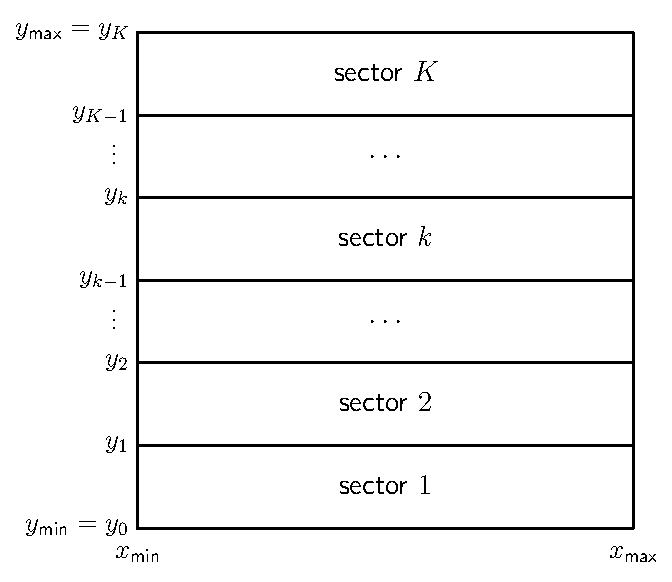
\includegraphics[width=.6\textwidth]{img/chapter3/2dsectors.pdf}
        \caption{\label{fig:c3_2dsectors} An illustration of the split in sectors along the $y$-axis for the domain $[\xmin, \xmax]\times[\ymin, \ymax]$.}
    \end{center}
\end{figure}

On each sector $k$ (with domain $[\xmin, \xmax]\times[y_{k-1}, y_k]$) a solution $\psi(x, y)$ will be approximated as a linear combination of the first $N$ basis functions:
\begin{equation}\label{equ:c3_lincomb_basis}
    \psi(x, y) \approx \sum_{i=1}^{N} b_i^{(k)}(x) c_i^{(k)}(y) = \transpose{{\vb{b}^{(k)}}}(x) \, \vb{c}^{(k)}(y) \text{.}
\end{equation}

The well-chosen basis $\left\{b_i^{(k)}\right\}$ Ixaru proposes can be calculated from the one dimensional Schrödinger equation. Let $b_i^{(k)}(x)$ be defined as the $i^\text{th}$ eigenfunction of the eigenvalue problem
$$
    -\pdv[2]{b_i^{(k)}}{x} + \bar{V}^{(k)}(x)b_i^{(k)}(x) = \lambda_i^{(k)} b_i^{(k)}(x)
$$
with boundary conditions $b_i^{(k)}(\xmin) = b_i^{(k)}(\xmax) = 0$. The function $\bar{V}^{(k)}(x)$ is a constant (in the $y$-direction) approximation of the potential $V$ on the $k^\text{th}$ sector. Ixaru proposes $\bar{V}^{(k)}(x) := V\left(x, \frac{y_{k-1} + y_k}{2}\right)$, we will later remark that other choices can be defended as well.

Just like the CP-methods, this new method employs shooting to locate the eigenvalues. For this, for a fixed value of $E$, formulae are needed to propagate solutions from the bottom of the domain (along $y = \ymin$) upwards, and from the top of the domain ($y = \ymax$) downwards. So, given a solution at the beginning of sector $k$ expressed in the basis $b_i^{(k)}$:
$ \psi(x, y_{k-1}) = \sum_{i=1}^{N} b_i^{(k)}(x)\, c_i^{(k)}(y_{k-1}) $, an expression is constructed to compute $c^{(k)}_i(y_k)$ at the end of the sector. Substituting \eqref{equ:c3_lincomb_basis} into \eqref{equ:c3_schrodinger_2d} gives rise to

\begin{equation}\label{equ:c3_coupled_system}
    -\pdv[2]{\vb{c}^{(k)}}{y} + \vb{V}^{(k)}(y) \vb{c}^{(k)}(y) = E \vb{c}^{(k)}(y) \text{.}
\end{equation}

In this expression $\vb{V}^{(k)}$ is an $N\times N$ matrix dependent on $y$:
\begin{equation}\label{equ:c3_v_matrix}
    \vb{V}^{(k)}_{ij}(y) = \int_{\xmin}^{\xmax} b_i^{(k)}(x) b_j^{(k)}(x) \left(V(x, y) - \bar{V}^{(k)}(x)\right) \dd x + \delta_{ij} \lambda_i^{(k)} \text{.}
\end{equation}

The system of ordinary differential equations given in \eqref{equ:c3_coupled_system} is a coupled system of Schrö\-dinger equations. For coupled systems, there are well-known CP-methods available \cite{ledoux_numerical_2007a,ixaru_lilix_2002}, with various implementations.

For the accurate computation of the integral in \eqref{equ:c3_v_matrix} we have developed specialized formulae. These will be presented later on in section \ref{sec:c3_calculate_vk}.

To be able to propagate a solution along the whole domain it is vital to have an expression to transfer solutions between consecutive sectors. To have continuous and continuously differentiable solutions, this property should also exist on the transition line between sectors. Therefore,
\begin{align*}
    \transpose{\vb{b}^{(k)}}(x) \, \vb{c}^{(k)}(y_k)                   & =\, \transpose{\vb{b}^{(k+1)}}(x) \, \vb{c}^{(k+1)}(y_k)                   \\
    \text{and}\quad
    \transpose{\vb{b}^{(k)}}(x)\,\pdv{\vb{c}^{(k)}}{y}\left(y_k\right) & = \transpose{\vb{b}^{(k+1)}}(x)\,\pdv[]{\vb{c}^{(k+1)}}{y}\left(y_k\right)
\end{align*}
should hold for all values of $x$. Multiplying both sides with $b_i^{(k)}$ and integrating along the $x$-axis for each $i \in \{1, \dots, N\}$, gives
\begin{align*}
    \vb{c}^{(k+1)}(y_k)                       & = \vb{M}^{(k)} \vb{c}^{(k)}(y_k)                       \\
    \pdv[]{\vb{c}^{(k+1)}}{y}\left(y_k\right) & = \vb{M}^{(k)} \pdv[]{\vb{c}^{(k)}}{y}\left(y_k\right)
\end{align*}
with
$$
    \vb{M}^{(k)}_{ij} = \bra{b_{i}^{(k)}}\ket{b_{j}^{(k+1)}} = \int_\xmin^\xmax b_i^{(k)}(x) b_j^{(k+1)}(x) \dd x \text{.}
$$
This is in the assumption that the orthogonal basis $\left\{b_i^{(k)}(x)\right\}$ is normalized $\bra{b_{i}^{(k)}}\ket{b_{j}^{(k)}} = \delta_{ij}$. In the infinite case this matrix $\vb{M}^{(k)}$ is orthogonal. In practice $N$ has to be finite, and $\vb{M}^{(k)}$ is in general no longer orthogonal. Intuitively this means that some information about the solution is lost when transitioning between sectors. This is a minor drawback, inherent to this method.

With these tools available, all that is left is to formalize how the shooting can be executed. Instead of propagating with a single starting condition (i.e. a column vector $\vb{c}^{1}(\ymin)$) all possible initial values (for vanishing boundary conditions) are propagated at once.
$$
    \begin{matrix}
        \vb{C}^{(1)}(\ymin) = \vb{0}_{N\times N} &            & \pdv[]{\vb{C}^{(1)}}{y}\left(\ymin\right) = \vb{I}_{N\times N} \\
                                                 & \text{and} &                                                                \\
        \vb{C}^{(K)}(\ymax) = \vb{0}_{N\times N} &            & \pdv[]{\vb{C}^{(K)}}{y}\left(\ymax\right) = \vb{I}_{N\times N}
    \end{matrix}
$$

In the matching point $y_m$, solutions are found. Since solutions have to be continuous and continuously differentiable, a `matching' condition can be formulated.  Let us define $\Cbottom$ and $\Cbottom'$ to be the values of $\vb{c}^{(m)}(y_m)$ and $\pdv[]{\vb{c}^{(m)}}{y}\left(y_m\right)$ respectively when propagated from the bottom of the domain upwards. Analogous $\Ctop$ and $\Ctop'$ can be defined. Now the value $E$ is an eigenvalue of the original problem if and only if there exists vectors $\ubottom$ and $\utop$ such that
\begin{align*}
    \Cbottom \cdot \ubottom                   & = \Ctop \cdot \utop           \\
    \text{and }\quad \Cbottom' \cdot \ubottom & = \Ctop' \cdot \utop \text{.}
\end{align*}
This is equivalent with saying $E$ is an eigenvalue of \eqref{equ:c3_schrodinger_2d} if and only if the mismatch matrix
\begin{equation}\label{equ:c3_psi_e}
    \vb{\Phi}(E) := \Cbottom'\Cbottom^{-1} - \Ctop'\Ctop^{-1}
\end{equation}
has a zero eigenvalue. Note that the multiplicity of the zero eigenvalue of this matrix is the same as the multiplicity of $E$ as an eigenvalue of \eqref{equ:c3_schrodinger_2d}. In the original article no details are given about how one should find the values of $E$ for which the matrix $\vb{\Phi}(E)$ becomes singular. Later, in section \ref{sec:c3_locating_e}, we will present our method for finding those values. In section \ref{sec:c3_index_of_e}, we will go even further and demonstrate a technique which allows to determine the index of the eigenvalue in question.

This concludes our overview of the method described by Ixaru in \cite{ixaru_new_2010}. There are a few differences between our overview and the method as described in \cite{ixaru_new_2010}. Most notably, as stated in the beginning, we have swapped the roles of $x$ and $y$. Ixaru split the domain in sectors along the $x$-axis, while we think it is more natural to apply the split along the $y$-axis\footnote{The main reason for this change in notation is to make the recursive nature of this method apparent. In future work we use this method to also solve the 3d time-independent Schrödinger equation. For this we split the domain along the $z$-axis, and solve on each sector the 2d Schrödinger equation in the $x\,y$-plane. For each of these 2d equations we split the domain along the $y$-axis, and solve the one dimensional Schrödinger equation along the $x$-axis.}. But this difference is only notational and does not change anything fundamental about the method.

\section{Our improvements}

In \cite{ixaru_new_2010}, Ixaru has presented a new promising method. As we have seen with the rise of CP-methods for the one-dimensional Sturm-Liouville equation, research builds upon previous work. With this in mind we have identified some possibilities where Ixaru's method can be expanded or improved. This section follows primarily the work done in \cite{baeyens_fast_2020}.

The first addition we have identified is implementing a robust algorithm to determine the eigenvalues themselves.

\subsection{Locating eigenvalues}\label{sec:c3_locating_e}

In \cite{ixaru_new_2010}, it is mentioned that the eigenvalues correspond to the values $E$ for which \eqref{equ:c3_psi_e} becomes singular. The suggestion is that the eigenvalues of this matrix are zero in when $E$ is an eigenvalue of \eqref{equ:c3_schrodinger_2d}. Nothing further is present on how these values for $E$ should be found.

In the literature many methods to find roots of functions are available. In introductory textbooks to scientific computing (e.g. \cite[Chapter~5]{heath_scientific_2002}), the most well-known methods are presented. One of the easiest to implement is the method of interval bisection. In this method the root of a scalar function $f : \RR \to \RR$ is determined by continuously halving a search interval. The position of the root can be tracked by ensuring the function $f$ has different sign on the boundary of the search interval. This requires that an initial guess for the interval already contains one root. But also, notice that the method will not work when the initial search interval contains more than one root, of a root with higher multiplicity.

Another well-known technique is Newton's method. Here, the root of a scalar function $f$ can be approximated by iterating the following scheme:
$$
    x_{n+1} = x_n - \frac{f(x_n)}{f'(x_n)}\text{.}
$$
For single roots, this method has a faster rate of convergence. Choosing initial values is also easier, because a value $x_0$ should be chosen only to be `sufficiently close' to a true root. One of the biggest drawbacks of this method is that the derivative of $f(x)$ should be available. For complicated functions, this can be difficult. Extensions of this method exist for which the derivative is not necessary, the secant method for example.

In all these well-known methods, the problem is that they only can be used to find a single root, not all roots. Furthermore, they only work on scalar function $\RR \to \RR$ or vector-functions for which roots are uniquely defined $\RR^n \to \RR^n$. In our case, we are interested in when any of the eigenvalues of $\eqref{equ:c3_psi_e}$ become zero. This does not map directly on any of these classical root-finding algorithms.

To combat these issues with the classical algorithms, we propose a light modification to Newton's method. Suppose an inaccurate approximation $E_0$ of an eigenvalue of the Schrödinger equation \eqref{equ:c3_schrodinger_2d} is given. Starting from this approximation we want a fast converging algorithm to find the true eigenvalue $E$. As stated earlier, $E$ is an eigenvalue if and only if it is a value such that $\vb{\Phi}(E)$ is singular, as defined by \eqref{equ:c3_psi_e}. In other words, the matrix $\vb{\Phi}(E)$ has to have a zero eigenvalue.

In Newton's method the derivative of the value in question should be available. Fortunately, in \cite{ixaru_lilix_2002} and also in \cite{ledoux_cpmp_2006} procedures are available to compute the derivative of solutions with respect to $E$. In our case, this means that the matrices
$$
    \pdv[]{\Cbottom}{E}, \pdv[]{\Cbottom'}{E}, \pdv[]{\Ctop}{E} \text{ and } \pdv[]{\Ctop'}{E}
$$
are available. This allows us to also compute the derivative of $\vb{\Phi}$ itself.
\begin{align*}
    \pdv{\vb{\Phi}}{E} = & \left(\pdv{\Cbottom'}{E} - \Cbottom'\Cbottom^{-1}\pdv{\Cbottom}{E}\right) \Cbottom^{-1} \\
                         & - \left(\pdv{\Ctop'}{E} - \Ctop'\Ctop^{-1}\pdv{\Ctop}{E}\right) \Ctop^{-1}
\end{align*}

Because we want to find roots within the eigenvalues of $\vb{\Phi}$, it is also valuable to be able to compute the derivative of an eigenvalue, with respect to $\vb{E}$. The derivatives of the eigenvalues of matrix-function are already known for a long time \cite{lancaster_eigenvalues_1964}.

\begin{theorem}[Lancaster 1964]\label{the:c3_eigenvalue_derivative}
    Let $\vb{A}(x)$ be a matrix functions $\mathbb{C} \to \mathbb{C}^{n\times n}$ such that each coefficient is continuously differentiable with respect to $x$ in the point $x_0$. Furthermore, assume $\vb{A}(x_0)$ to be diagonalizable\footnote{In \cite{lancaster_eigenvalues_1964}, it is noted that different, less stringent, assumptions may be made on the structure of $\vb{A}(x)$: ``This is equivalent to saying that every eigenvalue of [$\vb{A}(x_0)$] has only linear elementary divisors; or that [$\vb{A}(x_0)$] is diagonable, non-derogatory, non-defective, or similar to a diagonal matrix. This assumption could be replaced by the less restrictive condition that only the eigenvalue [$\lambda$] should have linear elementary divisors.''}.

    Let $\lambda$ be a simple eigenvalue of $\vb{A}(x_0)$ with left and right eigenvalues $\vb{v}$, $\vb{u}$ respectively. It now holds that
    $$
        \left(\dv[]{\lambda}{x}\right)_{x=x_0} = \frac{1}{\transpose{\vb{v}}\vb{u}} \left(\transpose{\vb{v}}\dv[]{\vb{A}}{x} \vb{u} \right)_{x=x_0}\text{,}
    $$
    where $\dv[]{\vb{A}}{x}$ is the matrix with, as each coefficient, the derivative of the corresponding coefficient of $\vb{A}(x)$ with respect to $x$.

\end{theorem}
\begin{proof}
    As $\vb{u}$ and $\vb{v}$ are right, respectively left, eigenvectors corresponding to the eigenvalue $\lambda$ it follows that:
    \begin{equation}\label{equ:c3_eigenvalue_derivative_equ1}
        \transpose{\vb{v}}\vb{A}(x_0)\vb{u}  = \lambda \transpose{\vb{v}}\vb{u}\text{.}
    \end{equation}
    Because all involved variables are dependent on $x$, and we will only take the value (or the value of the derivative) in $x_0$, we will, to ease notation, omit this $x$ dependency and implied evaluation in the point $x_0$. Furthermore, we will denote the derivative with respect to $x$ with a prime $'$. This allows us to write down the derivative of both sides of \eqref{equ:c3_eigenvalue_derivative_equ1}. These derivatives can further be simplified by using the product rule when applied to matrix multiplications:
    \begin{align*}
        \left(\transpose{\vb{v}}\vb{A}(x_0)\vb{u}\right)'                                                                    & = \left(\lambda \transpose{\vb{v}}\vb{u}\right)'                                                                      \\
        \implies \quad {\transpose{\vb{v}}}'\vb{A}\vb{u} + \transpose{\vb{v}}\vb{A}'\vb{u} + \transpose{\vb{v}}\vb{A}\vb{u}' & = \lambda' \transpose{\vb{v}}\vb{u} + \lambda {\transpose{\vb{v}}}'\vb{u} + \lambda \transpose{\vb{v}}\vb{u}'\text{.}
    \end{align*}
    Using that $\vb{u}$ and $\vb{v}$ are eigenvectors ($\vb{A} \vb{u} = \lambda \vb{u}$ and $\transpose{\vb{v}}\vb{A} = \lambda \transpose{\vb{v}}$), gives us the required expression:
    \begin{align*}
        \transpose{\vb{v}}\vb{A}'\vb{u} & = \lambda' \transpose{\vb{v}}\vb{u}                                         \\
        \implies \quad \lambda'         & = \frac{\transpose{\vb{v}}\vb{A}'\vb{u}}{\transpose{\vb{v}}\vb{u}} \text{.}
    \end{align*}
\end{proof}

Some care should be taken when two eigenvalues coincide. In \cite{lancaster_eigenvalues_1964}, this is handled by considering the left and right eigenvector space corresponding to the multiple eigenvalue. But since we are dealing with only numerical results this (almost) never happens. Theorem \ref{the:c3_eigenvalue_derivative} applied to $\vb{\Phi}(E)$ gives, with left and right eigenvectors, $\vb{v}$ and $\vb{u}$ respectively, corresponding to the eigenvalue $\lambda$:
$$
    \pdv{\lambda}{E} = \frac{1}{\transpose{\vb{v}}\vb{u}}\transpose{\vb{v}} \pdv{\vb{\Phi}}{E} \vb{u} \text{.}
$$

With values for all these derivatives, all tools are available to formulate our proposed modified Newton's scheme, to converge a crude initial guess $E_0$ to a true eigenvalue of \eqref{equ:c3_schrodinger_2d}. To simplify the notation we introduce the matrix-operator $\eigs$ which returns the set of eigenvalues of a matrix. This operator is defined on the $n \times n$-matrix $\vb{A}$ as
$$
    \eigs(\vb{A}) := \left\{\lambda \in \CC \, | \, \exists \vb{u} \in \CC^n : \vb{A} \vb{u} = \lambda \vb{u} \right\}\text{.}
$$

Now, we define the scalar function $f(E) : \RR \to \RR$ as {\color{red}To do: proof that $\vb{\Phi}(E)$ has only real eigenvalues.}
\begin{equation}\label{equ:c3_mismatch_newton_function}
    f(E) = \argmin_{\lambda \in \eigs(\vb{\Phi(E)}) \cap \RR} \left|\frac{\lambda}{\pdv*[]{\lambda}{E}}\right|\text{.}
\end{equation}

On this function $f(E)$ the classical Newton's method can be used. Note that this function is constructed such that in each step the eigenvalue with the closest, possible root will be selected.

\subsubsection{A numerical example}

To provide some intuition about the eigenvalues $\lambda$ of the mismatch matrix $\vb{\Phi}(E)$ we will analyze a numerical example. Consider the two-dimensional time-independent Schrödinger equation with potential function
\begin{equation}\label{equ:c3_mismatch_ixaru}
    V(x, y) = (1+x^2)(1+y^2)
\end{equation}
on the domain $[-5.5; 5.5] \times [-5.5; 5.5]$ with homogeneous Dirichlet boundary conditions. This problem is also the numerical example from Ixaru's work \cite{ixaru_new_2010}.

\begin{figure}
    \centering
    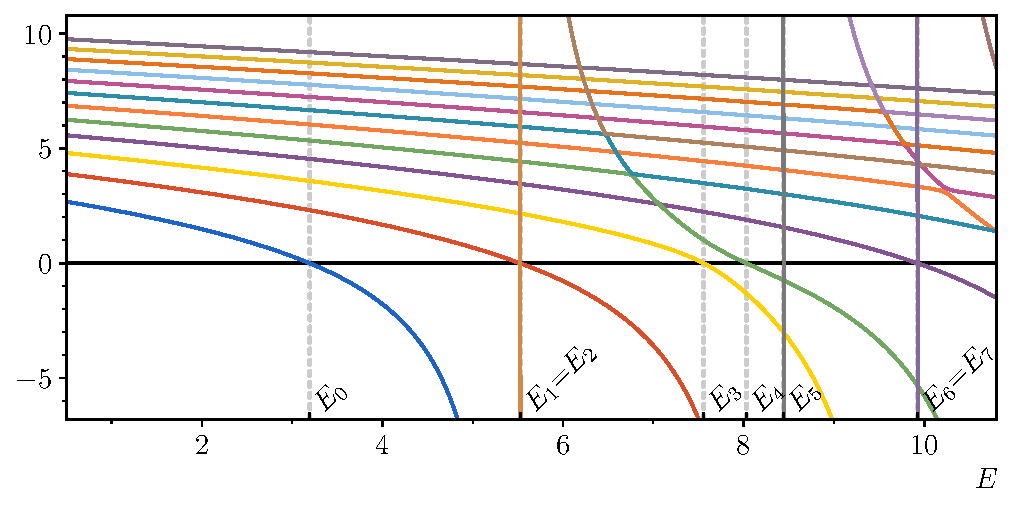
\includegraphics[width=\textwidth]{img/chapter3/mismatch_rainbow.pdf}
    \caption{\label{fig:c3_mismatch_rainbow} Each of the eigenvalues $\lambda$ of the mismatch matrix $\vb{\Phi}(E)$ of the Schrödinger problem \eqref{equ:c3_mismatch_ixaru} as a function of $E$. The true eigenvalues of this problem are indicated with $E_0$, $E_1$, $\dots$ The lines are colored and continued to aid in the clarity of this illustration. But, do notice that this is only a best guess approximation.}
\end{figure}

Throughout this research, one of the first graphs which we studied can be found in figure \ref{fig:c3_mismatch_rainbow}. Here all eigenvalues of the mismatch matrix $\vb{\Psi}(E)$ are plotted. For each value of $E$, $\vb{\Psi}(E)$ has the same number of eigenvalues ({\color{red}To do: only if the eigenvalues are real.}) as the chosen basis size $N$, as described in \ref{sec:c3_ixarus_method}. Upon seeing this graph, it is easy to say, that one can `follow' the trajectory of a single eigenvalue as $E$ changes. In reality, this is not easy at all. Sometimes two eigenvalue curves intersect, other times they barely avoid each other, and seemingly switch which curve they follow. Following the lowest eigenvalue $\lambda_0$, will  not result in a nice smooth curve, since this value can reach vertical asymptotes.

These difficulties and nuances are hidden away behind the colors and seemingly continuous lines present in figure \ref{fig:c3_mismatch_rainbow}. Practically, this graph is generated from the eigenvalues (and their derivatives) of $\vb{\Phi}(E)$ for $\numprint{10000}$ values of $E$. Two eigenvalues $\lambda^{(i)}_j$, $\lambda^{(i+1)}_k$  for two adjacent values $E_{i}$ and $E_{i+1}$, are determined to correspond to the same curve (and thus get the same color) if
$$ \lambda^{(i)}_j \approx \lambda^{(i+1)}_k - (E_{i+1} - E_i) \dv[]{\lambda^{(i+1)}_k}{E} $$
is sufficiently accurate.

\begin{figure}
    \centering
    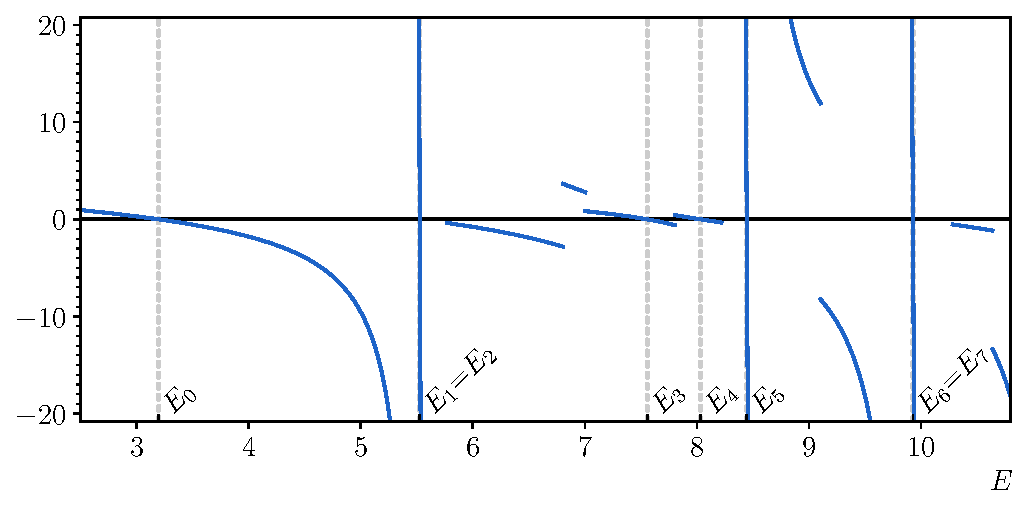
\includegraphics[width=\textwidth]{img/chapter3/mismatch_newton.pdf}
    \caption{\label{fig:c3_mismatch_newton} The function \eqref{equ:c3_mismatch_newton_function}, derived from problem \eqref{equ:c3_mismatch_ixaru}, is plotted. Notice that this graph can also be found as a part of figure \ref{fig:c3_mismatch_rainbow}. At first glance, the striking vertical lines may be assumed to be asymptotes. This is not the case, in these regions $f(E)$ changes very rapidly.}
\end{figure}

In figure \ref{fig:c3_mismatch_newton} the graph of the function $f(E)$ from equation \eqref{equ:c3_mismatch_newton_function} is plotted. Comparing this with figure \ref{fig:c3_mismatch_rainbow}, allows us to get an intuitive understanding of our application of Newton's method. But as can be seen in figure \ref{fig:c3_mismatch_newton}, this method is not perfect. The region in which eigenvalue $E_5$ can be detected is relatively small. If the more straightforward $f(x) = \argmin_{\lambda \in \eigs(\vb{\Phi(E)}) \cap \RR} \left|\lambda\right|$ was used different, this region would be even smaller. But still, numerically it would be very unlikely to stumble upon this region, to detect that an eigenvalue was missing. For this reason we have developed a robust way to determine the number of an eigenvalue less than the value $E$. This allows us to detect these missing values, and locate them. This technique will be studied in section \ref{sec:c3_index_of_e}.

\subsection{Calculation of \texorpdfstring{$\vb{V}^{(k)}(y)$}{Vk(y)}}\label{sec:c3_calculate_vk}

Another improvement we have made can be found in the calculation of the matrix $\vb{V}^{(k)}(y)$ with the formula in \eqref{equ:c3_v_matrix}. When one wants to implement this formula accurately, some considerations have to be made. As the formula consist of an integral with a relatively complicated integrand, we have to consider in which points this integrand is known. Furthermore, evaluating more points is non-trivial. In Ixaru's work \cite{ixaru_new_2010} it was not even possible to evaluate this integrand in more points. The values were only known in the mesh points of SLCPM12.

Because only a few values of the integrand, were known Ixaru has developed a particular exponentially fitted quadrature formula based upon \cite[Section~2.4]{ixaru_exponential_2004}. This method uses the exponential behavior of $b_i^{(k)}(x)$ and $b_j^{(k)}(x)$ the known approximate frequency to build specialized formulae. Because the derivatives with respect to $x$ of $b_i^{(k)}(x)$ and $b_j^{(k)}(x)$ are known, and those of $V(x, y)$ and $\bar{V}^{(k)}(x)$ can be estimated, these values are also used.

In our case, the story is quite different. Because of our improvements to Matslise, we can improve accuracy even further. In particular, the computation of $b_i^{(k)}(x)$ is now efficiently possible in arbitrary points. This allows us to use off the shelf quadrature formulae, to ensure accuracy. As this was only a first test to approximate $\vb{V}^{(k)}(x)$, we did not use specialized exponentially fitted methods. When profiling our implementation we found that the time to execute these quadrature formulae was almost negligible.

So in practice, there was little need to improve even further, with more complicated quadrature formulae. But, as numerical analysts, we were still curious if some more fundamental improvements were possible. After all, the eigenfunctions $b_i^{(k)}(x)$, are approximated piecewise by a truncated series in the step size $\delta$ and the special functions $\eta_{-1}$, $\eta_{0}$, $\dots$ But also, the function $\bar{V}^{(k)}$ is already approximated by a sixteenth degree polynomial. The only `wildcard', so to speak, is the unknown general function $V(x, y)$, for a fixed value of $y$. In the middle of the $k^\text{th}$ sector, this function is approximated piecewise. As such, it is reasonable to assume, that a piecewise sixteenth degree polynomial can be accurately fitted on this function $V(x, y)$, if the same pieces as for $\bar{V}^{(k)}$ are used.


{\color{red} To do: writing more and include appendix from reinventing-2d-schrodinger}


\section{Determining the index of eigenvalues}\label{sec:c3_index_of_e}

\begin{theorem}[Counting eigenvalues]
    \label{the:c3_counting_eigenvalues}
\end{theorem}

\subsection{A test on a more exotic domain}

As a numerical demonstration that this theorem is true for more domains than only the rectangle, we demonstrate it on a series of moon-shaped domains. For this, define the transformation $T:[-\frac{\pi}{2}, \frac{\pi}{2}] \times [-1, 1] \to \RR^2$ as:
\begin{equation}\label{equ:c3_disc_transformation}
    T(\alpha, t) = \begin{pmatrix}
        \cot(\alpha) \sin(t \alpha) \\
        \frac{1}{\sin(\alpha)} - \cot(\alpha) \cos(t \alpha)
    \end{pmatrix}\text{.}
\end{equation}
Strictly speaking, for $\alpha = 0$,  $T(\alpha, t)$ is undefined. In these points the limit $\lim_{\alpha \to 0} T(\alpha, t)$ should be considered. In figure \ref{fig:c3_disc_transformation} this transformation is visualized. Note that when $t$ is limited to $[-1, 2\epsilon -1]$ the transformation results in a moon-shape.

\begin{figure}
    \begin{center}
        \begin{minipage}{.53\textwidth}
            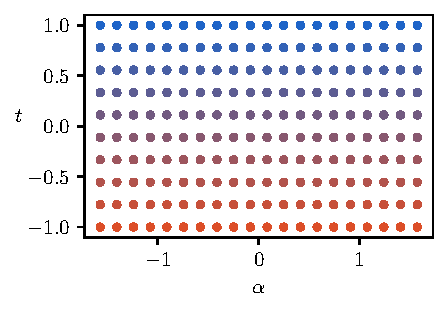
\includegraphics[scale=.75]{img/chapter3/on_disc/disc_original.pdf}%
        \end{minipage}\begin{minipage}{.05\textwidth}\begin{center}
                \Large $ \xrightarrow{T} $
            \end{center}
        \end{minipage}\begin{minipage}{.42\textwidth}\centering
            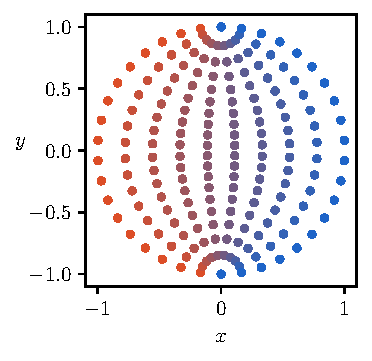
\includegraphics[scale=.75]{img/chapter3/on_disc/disc_transformed.pdf}
        \end{minipage}
    \end{center}
    \caption{The transformation $T(\alpha, t)$ from \eqref{equ:c3_disc_transformation} is applied to a grid of points.}
    \label{fig:c3_disc_transformation}
\end{figure}



To demonstrate the effectiveness of theorem \ref{the:c3_counting_eigenvalues}, we will consider the series of continuous subdomains
$$
    \Omega_\epsilon = \left\{T(\alpha, t) | \forall \alpha \in \left[-\frac{\pi}{2}, \frac{\pi}{2}\right], \forall t \in [-1, 2\epsilon - 1]  \right\}\text{.}
$$
On these subdomains $\Omega_\epsilon$ we will approximate the eigenvalues of the Schrödinger equation with homogeneous Dirichlet boundary conditions. Subsequently, these eigenvalues can be compared to the eigenvalues on the unit disc. The theorem promises that for an eigenvalue $\lambda_i$ on the unit disc, exactly $i$ subdomains can be found on which this $\lambda_i$ is also an eigenvalue.

First, let us clearly define which Schrödinger problem we are solving: Find the eigenvalues $\lambda$ with corresponding eigenfunction $\psi(x, y) \in \Omega_\epsilon \to \RR$ for which
\begin{equation}\label{equ:c3_disc_schrodinger}
    -\nabla^2 \psi(x, y) = \lambda \psi(x, y)
\end{equation}
holds. As boundary conditions we impose $\psi(x, y) = 0$ on the boundary $\delta \Omega$.

\subsubsection{Transforming the problem onto a rectangular domain}

Approximating solutions for the eigenvalues of \eqref{equ:c3_disc_schrodinger} on such an exotic domain $\Omega_\epsilon$ is not a trivial task. In principle, this problem could be seen as solving the Schrödinger equation on $[-1,1]^2$ with the potential
$$
    V(x, y) = \begin{cases}
        0       & \text{if $(x, y)\in \Omega_\epsilon$} \\
        +\infty & \text{otherwise}
    \end{cases} {}\text{.}
$$
But numerically, this does not make the problem easier. Yes, the rectangular domain would allow us to employ the earlier developed method. But on the other hand, the potential becomes infinite, which is very difficult to implement with sufficiently high accuracies. Also, Ixaru's method has difficulties with non-continuous potentials.

We propose another technique. We can transform equation \eqref{equ:c3_disc_schrodinger} from these moon-shaped domains to a more manageable rectangular domain. The cost of this transformation is that \eqref{equ:c3_disc_schrodinger} will no longer be a Schrödinger equation.

As earlier stated, the transformation we will apply is the function $(x, y) = T(\alpha, t)$. To formalize this, we introduce the function $\phi(\alpha, t)$ as
$$
    \phi(\alpha, t) = \psi(T(\alpha, t))\text{.}
$$
With this transformation the Schrödinger equation \eqref{equ:c3_disc_schrodinger} transforms into
\begin{equation}\label{equ:c3_disc_schrodinger_transformed}
    -\mathcal{D}\phi(\alpha, t) = \lambda\phi(\alpha, t)
\end{equation}
with $\phi(\alpha, t)$ defined on the domain $\Xi_\epsilon = \left[-\frac{\pi}{2}, \frac{\pi}{2}\right] \times [-1, 2\epsilon - 1]$. Note that $T(\Xi_\epsilon) = \Omega_\epsilon$. As boundary conditions we impose $\phi(\alpha, t) = 0$ if $(\alpha, t) \in \delta\Xi_\epsilon$ on the boundary. In this expression $\mathcal{D}$ is the differential operator corresponding to $\nabla^2\psi(x, y)$. Calculating this operator by hand is tedious, therefore we will use \sage to do the symbolic heavy lifting for us. To be able to work with the operator $\mathcal{D}$, we first need a procedure to compute it. To ease notation we will denote $T(\alpha, t) = (T^{x}(\alpha, t), T^{y}(\alpha, t))$, and omit the arguments to the functions $\phi$, $\psi$ and $T$. Derivatives will be denoted as $\phi_\alpha = \pdv[]{\phi}{\alpha}$ and $\phi_{\alpha\alpha} = \pdv[2]{\phi}{\alpha}$. We compute all first and second derivatives of $\phi(\alpha, t)$.
\begin{equation}\label{equ:disc_transformation_derivatives}
    \begin{cases}
        \phi_\alpha = \psi_x T^x_\alpha + \psi_y T^y_\alpha                                                                                                                   \\
        \phi_t = \psi_x T^x_t + \psi_y T^y_t                                                                                                                                  \\
        \phi_{\alpha\alpha} = \psi_x T^x_{\alpha\alpha} + \psi_y T^y_{\alpha\alpha} + \psi_{xx} (T^x_\alpha)^2 + 2 \psi_{xy} T^x_\alpha T^y_\alpha + \psi_{yy} (T^y_\alpha)^2 \\
        \phi_{\alpha t} = \psi_x T^x_{\alpha t} + \psi_y T^y_{\alpha t} + \psi_{xx} (T^x_\alpha)(T^x_t) + \psi_{xy} \left(T^x_\alpha T^y_t + T^x_t T^y_\alpha \right)         \\
        \quad\quad\quad\quad {} + \psi_{yy} (T^y_\alpha)(T^y_t)                                                                                                               \\
        \phi_{tt} = \psi_x T^x_{tt} + \psi_y T^y_{tt} + \psi_{xx} (T^x_t)^2 + 2 \psi_{xy} T^x_t T^y_t + \psi_{yy} (T^y_t)^2
    \end{cases}
\end{equation}

The question now is, can we isolate $\psi_{xx} + \psi_{yy}$ from the right-hand side of the system from \eqref{equ:disc_transformation_derivatives}? As this is a linear system in the derivatives of $\psi$, there is a unique linear combination $\vb{c}(\alpha, t) = (c^\alpha, c^t, c^{\alpha\alpha}, c^{\alpha t}, c^{tt})$ of rows such that:
$$
    c^\alpha \phi_\alpha + c^t\phi_t + c^{\alpha\alpha}\phi_{\alpha\alpha} + c^{\alpha t} \phi_{\alpha t} + c^{tt} \phi_{tt} = \psi_{xx} + \psi_{yy}\text{.}
$$

This linear combination allows us to finally determine the operator $\mathcal{D}$, and by extension the partial differential equation \eqref{equ:c3_disc_schrodinger} transforms into. Note that because $\vb{c}$ is dependent on $\alpha$ and $t$, that the operator $\mathcal{D}$ has this dependency as well.
$$
    \mathcal{D} = c^\alpha {\pdv[]{}{\alpha}} + c^t \pdv[]{}{t} + c^{\alpha\alpha} \pdv[]{}{\alpha\alpha} + c^{\alpha t} \pdv[]{}{\alpha t} + c^{tt} \pdv[]{}{tt}
$$

\subsubsection{A specialized numerical method}

Before we can analyze eigenvalues of \eqref{equ:c3_disc_schrodinger} or after transformation of the operator $-\mathcal{D}$ in relation to the domain $\Omega_\epsilon$, we still need a method to approximate these eigenvalues. For general partial differential equations with boundary conditions some standard techniques are available, \cite[Chapter~11]{heath_scientific_2018} contains an overview of some of these methods. Our choices include, but are not limited to a finite difference method, or a finite element method or a semidiscrete method with shooting. For our purposes a method which is easy to implement, yet gives reliable results will be the best choice. A simple finite difference scheme will be sufficient.

We will place an $n_\alpha \times n_t$ grid on the domain $\Xi_\epsilon$. This gives rise to the equidistant points $-\frac{pi}{2}=\alpha_0, \alpha_1, \dots, \alpha_{n_\alpha} = \frac{\pi}{2}$, and the points $-1 = t_0, t_1, \dots t_{n_t} = 1 - 2\epsilon$. The distances between two points are given by $h_\alpha = \frac{\pi}{n_\alpha}$ and $h_t = \frac{2\epsilon}{n_t}$. Because of the homogeneous Dirichlet boundary conditions $\phi_{0,j} = \phi_{n_\alpha,j} = \phi_{i, 0} = \phi_{i,n_t} = 0$ for all $i$ and $j$. These grid points allow us to write down approximations of first and second derivatives of $\phi(\alpha, t)$ in each of the grid points $\phi_{i, j} = \phi(\alpha_i, t_j)$.
\begin{align*}
    {\pdv[]{\phi}{\alpha}}(\alpha_i, t_j)    & = \frac{1}{2h_\alpha}\left( \phi_{i+1,j} - \phi_{i-1,j} \right)                                           \\
    {\pdv[]{\phi}{t}}(\alpha_i, t_j)         & = \frac{1}{2h_t}\left( \phi_{i,j+1} - \phi_{i,j-1} \right)                                                \\
    {\pdv[2]{\phi}{\alpha}}(\alpha_i, t_j)   & = \frac{1}{h_\alpha^2}\left( \phi_{i+1,j} - 2 \phi_{i,j} + \phi_{i-1,j} \right)                           \\
    {\pdv[]{\phi}{\alpha}{t}}(\alpha_i, t_j) & = \frac{1}{4h_\alpha h_t}\left( \phi_{i+1,j+1} - \phi_{i+1,j-1} - \phi_{i-1,j+1} + \phi_{i-1,j-1} \right) \\
    {\pdv[2]{\phi}{t}}(\alpha_i, t_j)        & = \frac{1}{h_t^2}\left( \phi_{i,j+1} - 2 \phi_{i,j} + \phi_{i,j-1} \right)
\end{align*}

When working with finite difference schemes, especially for a more  advanced operator such as $\mathcal{D}$, writing out all formulas becomes quite tedious. Therefore, it is much more comprehensive if we introduce some matrix notation. Let us denote the identity matrix of dimensions $n \times n$ as $\vb{I}_n$. Furthermore, a diagonal matrix with $a_1, \dots a_n$ on the diagonal will be denoted as $\diag_n(a_1, \dots, a_n)$, and an $n \times n$ tridiagonal Toeplitz matrix, with $c_{0}$ on the main diagonal, $c_{-1}$ below it and $c_1$ above it, will be denoted as $\tridiag_{n}(c_{-1}, c_{0}, c_1)$. To aid the finite difference approximations we introduce $\vb{D}^{(1)}_n = \frac{1}{2}\tridiag_n(-1,0,1)$ and $\vb{D}^{(2)}_n = \tridiag_n(1,-2,1)$

We will define the Kronecker product of a $k \times l$ matrix $\vb{A}$ and $m \times n$ matrix $\vb{B}$ as the $km \times ln$ block matrix:
$$
    \vb{A} \otimes \vb{B} := \begin{pmatrix}
        A_{1,1} \vb{B} & A_{1, 2} \vb{B} & \dots  & A_{1, l} \vb{B} \\
        A_{2,1} \vb{B} & A_{2, 2} \vb{B} & \dots  & A_{2, l} \vb{B} \\
        \vdots         & \vdots          & \ddots & \vdots          \\
        A_{k,1} \vb{B} & A_{k, 2} \vb{B} & \dots  & A_{k, l} \vb{B} \\
    \end{pmatrix}{}\text{.}
$$

To approximate \eqref{equ:c3_disc_schrodinger_transformed} as a matrix problem, we need to aggregate the grid points $\phi_{i,j}$ as a vector. For this we define
$$
    \vb*{\phi} := \transpose{\begin{pmatrix}
            \phi_{1,1}, \phi_{2,1}, \dots \phi_{n_\alpha-1, 1}, \phi_{1,2}, \dots \phi_{n_\alpha-1, n_t-1}
        \end{pmatrix}}\text{.}
$$
Also, to be able to write down $\mathcal{D}$ as a matrix operation we need to define
$$
    \vb{C}^{t} := \transpose{\begin{pmatrix}
            c^{t}(\alpha_1, t_1), c^{t}(\alpha_2, t_1) \dots c^{t}(\alpha_{n_\alpha-1}, t_1), c^{t}(\alpha_1, t_2), \dots c^{t}({\alpha_{n_\alpha-1}, t_{n_t-1}})
        \end{pmatrix}}\text{,}
$$
and analogous for $\vb{C}^{\alpha}$, $\vb{C}^{\alpha\alpha}$, $\vb{C}^{\alpha t}$ and $\vb{C}^{t t}$.

All this notation allows us to approximate \eqref{equ:c3_disc_schrodinger_transformed} as a matrix eigenvalue problem:
$$
    -\vb{M} \vb*{\phi} = \lambda \vb*{\phi}
$$
with
\begin{align*}
    \vb{M} = {} & \frac{1}{h_\alpha} \vb{C}^{\alpha} \left(\vb{I}_{n_t - 1}\otimes \vb{D}^{(1)}_{n_\alpha - 1} \right) + \frac{1}{h_t} \vb{C}^{t} \left(\vb{D}^{(1)}_{n_t - 1}  \otimes \vb{I}_{n_\alpha - 1}\right)                \\
                & {} + \frac{1}{h_\alpha^2} \vb{C}^{\alpha\alpha} \left(\vb{I}_{n_t - 1}\otimes \vb{D}^{(2)}_{n_\alpha - 1}\right) + \frac{1}{h_t^2} \vb{C}^{tt} \left(\vb{D}^{(2)}_{n_t - 1}  \otimes \vb{I}_{n_\alpha - 1}\right) \\
                & {} + \frac{1}{h_\alpha h_t} \vb{C}^{\alpha t} \left(\vb{I}_{n_t - 1}\otimes \vb{D}^{(1)}_{n_\alpha - 1} \right) \left( \vb{D}^{(1)}_{n_t - 1}  \otimes \vb{I}_{n_\alpha - 1} \right)\text{.}
\end{align*}

\subsubsection{Analysis of eigenvalues in relation to the domain}

Before applying this numerical method on different domains $\Omega_\epsilon$ it is valuable to first find the eigenvalues on the disc $\Omega_1$ itself. In many introductory textbooks to (partial) differential equations the study of the wave equation on a drum is considered. In most texts, if not all, the idea boils down to: with a transformation to polar coordinates and separation of variables this two-dimensional problem can be transformed into two one-dimensional problems. One of these can be solved directly, the other gives rise to the so-called Bessel functions.

Here we will give a brief overview of the symbolic calculations to solve
\begin{equation}\label{equ:c3_disc_before_polar}
    -\nabla^2 \psi(x, y) = \lambda \psi(x, y)
\end{equation}
on the unit disc $B(\vb{0}, 1)$, with homogeneous Dirichlet boundary conditions. For more details one could consult for example \cite[chapter~4]{asmar_partial_2005}. As stated we first transform \eqref{equ:c3_disc_before_polar} to polar coordinates. For this we pose $x = r\cos(\theta)$ and $y = r\sin(\theta)$, with $r \in [0,1]$ and $\theta \in [0, 2\pi]$. The solutions $u(r, \theta) := \psi(r\cos(\theta), r\sin(\theta))$ are now considered in the transformed domain. Applying the chain rule to $\nabla^2\psi$, yields the new equation
\begin{equation}\label{equ:c3_disc_after_polar}
    -{\pdv[2]{u}{r}} - \frac{1}{r}{\pdv[]{u}{r}} - \frac{1}{r^2} {\pdv[2]{u}{\theta}} = - \lambda u\text{.}
\end{equation}
The boundary conditions are likewise transformed: $u(1, \theta) = 0$ for all $\theta \in [0, 2\pi]$ and $u(r, 0) = u(r, 2\pi)$ and ${\pdv[]{u}{\theta}}(r, 0) = {\pdv[]{u}{\theta}}(r, 2\pi)$ for all $r \in [0, 1]$.

Now we use the method of separation of variables to transform \eqref{equ:c3_disc_after_polar} into two one-dimensional problems. For this, we separate $u(r, \theta) = R(r) \Theta(\theta)$ into a product of an $r$-dependent function and a $\theta$-dependent function. This allows us to write
$$
    -\frac{r^2 R''}{R} - \frac{rR'}{R} - \frac{\Theta''}{\Theta} = \lambda r^2 \text{.}
$$
Rearranging terms to an $r$-dependent side and a $\theta$-dependent side yields two separate equations
\begin{align*}
    \lambda r^2 + \frac{r^2 R''}{R} + \frac{rR'}{R} & = k & \text{and} &  & -\frac{\Theta''}{\Theta} & = k\text{,}
\end{align*}
with $k$ a constant and boundary conditions $R(1) = 0$, $\Theta(0) = \Theta(2\pi)$ and $\Theta'(0) = \Theta'(2\pi)$.

Solutions for $\Theta(\theta)$ can directly be found, as a solution of a linear second order differential equation with constant coefficients. Thus, $\Theta$ only has periodic solutions
$$
    \Theta(\theta) = A_m \cos(m\theta) + B_m \sin(m\theta)\text{,}
$$
if $k = m^2$ with $m \in \{0, 1, 2, \dots\}$. Note that if $m > 0$, there are two linear independent solutions for $\Theta$.

The differential equation for $R(r)$ becomes
$$
    r^2 R'' + r R + (\lambda r^2 - m^2)R = 0\text{.}
$$
We find that solutions to our equation can be written using the $m^\text{th}$ so-called Bessel function of the first kind $R(r) = J_m(r \sqrt{\lambda})$, for more details about these functions see for example \cite[section~4.7]{asmar_partial_2005}. These solutions only satisfy the boundary condition $R(1) = 0$, if and only if $\sqrt{\lambda}$ is a positive zero of $J_m$. If we denote $j_{m, n}$ as the $n^\text{th}$ positive root of the $m^\text{th}$ Bessel function $J_m$ we find that all eigenvalues of \eqref{equ:c3_disc_after_polar} and also of \eqref{equ:c3_disc_before_polar} are given as the squares of roots of the Bessel functions. So $\lambda = j_{m, n}^2$ is an eigenvalue of \eqref{equ:c3_disc_before_polar}. It is single eigenvalue if $m = 0$, otherwise it is a double eigenvalue. The following table contains the first ten eigenvalues, counted with multiplicity.

\begin{center}
    \bgroup
    \def\arraystretch{1.5}
    \begin{tabular}{r|cccccc}
        Eigenvalue       & $\lambda_0$ & $\lambda_{1,2}$ & $\lambda_{3,4}$ & $\lambda_{5}$ & $\lambda_{6,7}$ & $\lambda_{8,9}$ \\ \hline\hline
        Analytical value & $j_{0,1}^2$ & $j_{1,1}^2$     & $j_{2,1}^2$     & $j_{0,2}^2$   & $j_{3,1}^2$     & $j_{1,2}^2$     \\ \hline
        Numerical value  & $5.783$     & $14.68$         & $26.37$         & $30.47$       & $40.71$         & $49.22$
    \end{tabular}
    \egroup
\end{center}

With a numerical method to compute eigenvalues of the wave equation \eqref{equ:c3_disc_schrodinger} on moon-shaped domains $\Omega_\epsilon$, and a comprehensive analysis of the true eigenvalues of this equation on the disc $\Omega_1$, we are able to demonstrate theorem \ref{the:c3_counting_eigenvalues}.

\begin{figure}
    \begin{center}
        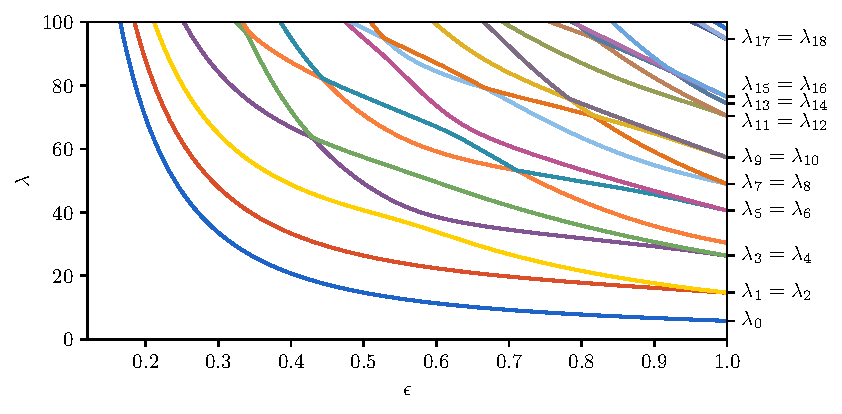
\includegraphics[width=\textwidth]{img/chapter3/on_disc/eigenvalues_flow.pdf}
        \caption{Eigenvalues in relation to $\epsilon$.}
        \label{fig:c3_disc_eigenvalues_flow}
    \end{center}
\end{figure}

By employing our numerical method on different domains $\Omega_\epsilon$ we can compute figure \ref{fig:c3_disc_eigenvalues_flow}. Here each line corresponds to a different eigenvalue. The lowest blue line visualizes the changes in the lowest eigenvalue according to the domain. For small domains $\epsilon \to 0$, this value becomes larger. The red line, right above the blue line corresponds to the eigenvalue with index $1$ of the wave equation on $\Omega_\epsilon$. For $\Omega_1$, this eigenvalue has a double multiplicity $\lambda_1 = \lambda_2$. But for all smaller domains, this degeneracy disappears, and $\lambda_1$ is a single eigenvalue. Which eigenvalue each line represent is marked on the right side. In accordance with theorem \ref{the:c3_counting_eigenvalues} all lines in figure \ref{fig:c3_disc_eigenvalues_flow} are continuous, decreasing and unbounded when $\epsilon \to 0$.


\begin{figure}
    \begin{center}
        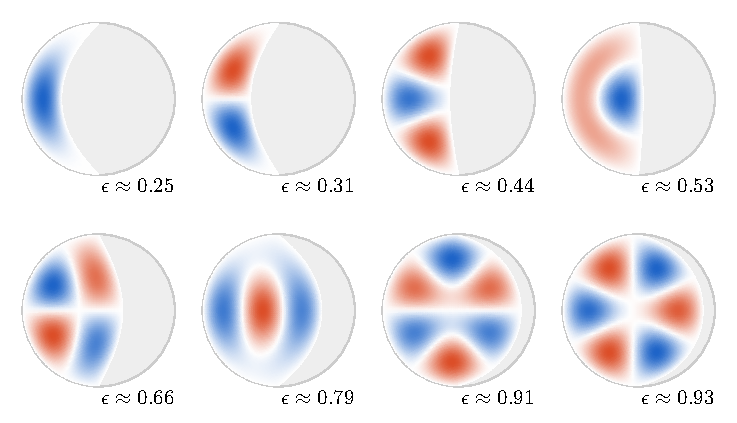
\includegraphics[width=\textwidth]{img/chapter3/on_disc/solutions.pdf}
        \caption{There are $8$ smaller moon shaped domains on which $\lambda = 45$ is an eigenvalue of the wave equation $-\nabla^2 \psi = \lambda \psi$ with homogeneous Dirichlet boundary conditions.}
        \label{fig:c3_disc_solutions}
    \end{center}
\end{figure}


Consider now the fixed value of $E = 45$. From the previous table we know that there are $8$ eigenvalues, counted with multiplicity, less than $E$. This means, following theorem \ref{the:c3_counting_eigenvalues}, there should be exactly $8$ moon shaped domains on which $E$ is also an eigenvalue. These eight domains, with the corresponding eigenfunction of $E = 45$, are plotted in figure \ref{fig:c3_disc_solutions}.

\section{Numerical experiments}

{\color{red} To do}

\section{Conclusions}

{\color{red} To do}

\begin{enumerate}
    \item accuracy
    \item run time
    \item numerical stability
    \item order estimates
    \item benefits vs. disadvantages
    \item possible future work
\end{enumerate}


\stopchapter
